\chapter{Characteristics of Neural Networks}\label{char_nn}
In this chapter, we will explore the characteristics of NN models we want to measure and analyse. For the rest of the paper, we will use the term \textit{characteristics} to identify all the metrics and properties of NNs which will have an influence on their performances in an actual deployment. The term is therefore an umbrella term for any type of measurable property which can influence the recognition of sugar beets. In the following sections we will give a through overview of each one of them with the main goal of understanding them. 

\section{Deep Neural Networks and Uncertainty}
As the scope of our investigation is to be able to recognize characteristics and find empirically their correlations in the field of sugar beet recognition, we need to be able to produce predictable and reliable results in order to pose foundation for our analysis. Although this is true in general terms, before we explore techniques to measure Neural Networks, it is important that we understand that we can not properly use the term ''predictability'' when discussing DNNs. \\
Due to the increased trust given by the advancements in recent years, DNNs are being applied in numerous different fields, as shown by the increasing number of peer review papers about Deep Learning (Fig. \ref{fig:annual_trend}), even the higher-risk ones 
like medical image analysis or autonomous vehicle control. \cite{gawlikowski2021survey}
\begin{figure}[h]
    \centering
    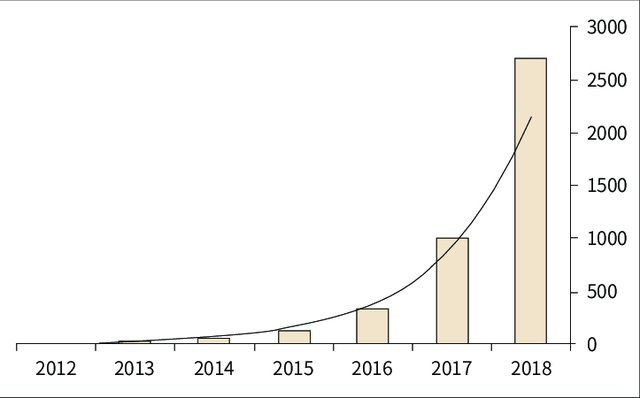
\includegraphics{img/Annual-trend-in-the-number-of-papers-related-to-deep-learning-in-the-medical-field_W640.jpg}
    \caption[Trend in publications about Deep Learning]{Trend in publications about Deep Learning  \cite{Number_of_DL_papers}}
    \label{fig:annual_trend}
\end{figure}


In such high-risk scenarios, DNNs should not only be highly accurate, as a mistake in detecting an obstacle could cause catastrophic consequences for the passengers, but also be trustworthy enough so that the probability of the predicted values reflects the ground truth. DNNs, however, are subjected to different source of uncertainty and errors. \textit{Galiwoski et al.} in \cite{gawlikowski2021survey} recognize five crucial factors which can cause uncertainty and errors in DNNs.\\\hfill

Those factors are:

\begin{enumerate}[label=\Roman*.]
    \item the variability in real world situations. 
    \item the errors inherent to the measurement systems,
    \item the errors in the architecture specification of the DNN,
    \item the errors in the training procedure of the DNN,
    \item the errors caused by unknown data.
\end{enumerate}
%In the next section, we will explore these factor in more details. Subsequently, we will reason about methods to reduce it and finally, in the third section, we will individuate methods to classify it. 
%\subsection{Factors causing Uncertainty}
We can model a neural network as a function $f$, parametrized by weight $\theta$, which maps a set of input $\mathbb{X}$ to a set of measurable outputs $\mathbb{Y}$, hence:
\begin{equation}
    f\theta : \mathbb{X} \rightarrow \mathbb{Y} \quad\quad\quad
    f\theta(x) = y
    \label{eq:DNN_model}
\end{equation}
In case of supervised learning, we also model the training set as $\mathcal{D} \subset \mathbb{D} = \mathbb{X} \times \mathbb{Y}$, where $\mathbb{X}$ is an instance space and $\mathbb{Y}$ the set of outcomes that can be associated with an instance (\cite{uncertainity_classi}), containing $N$ samples. A DNN trained in $\mathcal{D}$ can therefore predict a a corresponding target $f\theta(x^*) = y^*$.\\
During the data acquisition process, a measurement $x$ and a target variable $y$ are taken from space $\Omega$ to  represent a real world situation $\omega$. For example, $\omega$ could be a sugar beet, $y$ the label ''sugar beet'' and $x$ a picture of a sugar beet. The job of the DNN is therefore to predict the label from the image of the sugar beet (Eq n. \ref{eq:DNN_model}). In a real world situation, however, measurements could be potentially different from the ones used for training and this could influence the prediction of $y$. The source of this difference could be different lighting condition, different environmental condition or any other general conditions not taken into account when training. A new measurement generally is not part of the training set, hence $x^* \notin \mathcal{D}$.These differences in real world scenarios compared to the training set are called \textit{distribution shifts}(\cite{ovadia2019trust}) and DNN are very sensitive to that. Moreover, source of noise could also be individuated in errors in labelling. This is the first factor that can cause uncertainty, i.e. \textbf{the variability in real world situations}. \cite{gawlikowski2021survey}\\
In addition, it has to be taken into account that measurement devices are also subjected to noise due to defects or imprecision. This kind of noise is the second factor, i.e. \textbf{tthe errors inherent to the measurement systems}. \cite{gawlikowski2021survey}\\
We previously modelled a neural network simply as a function $f\theta$. Although in most applications DNN are treated similarly to how we modelled them, i.e. as a black box which takes as input some data and outputs a prediction, they have a certain structure with certain parameters to take care of. These parameters can be for example the amount of layer, the parameters which need to be configured and the chosen activation function. These configurations are up to the modeller and are the third cause of uncertainty in DNNs, i.e. \textbf{the errors in the architecture specification of the DNN}. \cite{gawlikowski2021survey}\\
A further source of uncertainty in DNNs is also related to the very own nature of DNNs. DNNs are not deterministic, rather they are stochastic\footnote{Stochastic is a synonym for randomness} in many ways : the order of data, the weight initialization or random regularization as augmentation or dropout. \cite{gawlikowski2021survey} Moreover, the stochastic gradient descent algorithm is widely use to optimize the learning process of DNNs. \cite{ruder2017overview}\\
Another version of the gradient descent algorithm which is also used is the mini-batch version, which selects random batches with aleatory size (called batch size) from the learning data-set to optimize the training process. \cite{ruder2017overview} This parameter, in addition to other ones like learning rate, and the number of training epochs, is also source of unpredictability in the DNN, as they could heavily change its performances  \\
The stochastic nature of DNN and the choices of the aforementioned parameters are the forth cause of uncertainty in DNNs : \textbf{the errors in the training procedure of the DNN}\\
Previously we modelled the training set as $\mathcal{D} \subset \mathbb{D}$, hence as being a subset of a certain domain $\mathbb{D}$. However, the realm of input which could be fed to a neural network is not limited to this domain, rather the DNN is trained to solve tasks with inputs belonging to this domain. Another source of uncertainty can be therefore an input which the DNN is not trained for, even though it is able to process it. For instance, if a DNN is trained to classify dogs from images, an image as input could also depict a bird. The last factor which could cause uncertainty is therefore the \textbf{errors caused by unknown data}. Such unknown data, could also be caused by highly noisy measurement devices, like a broken camera, and some researches show how easy is to fool DNN with images that are meaningless for us humans.\cite{nguyen2015deep} Fig.\ref{fig:fooling_DNN} depicts some examples of picture which could fool even the most advanced DNN. The figures on the top row could also be produced by random noise from a malfunctioning camera and yet could be classified as something else with an accuracy $\geq$ 99.6\%. \cite{nguyen2015deep}\\
\begin{figure}[htb]
    \centering
    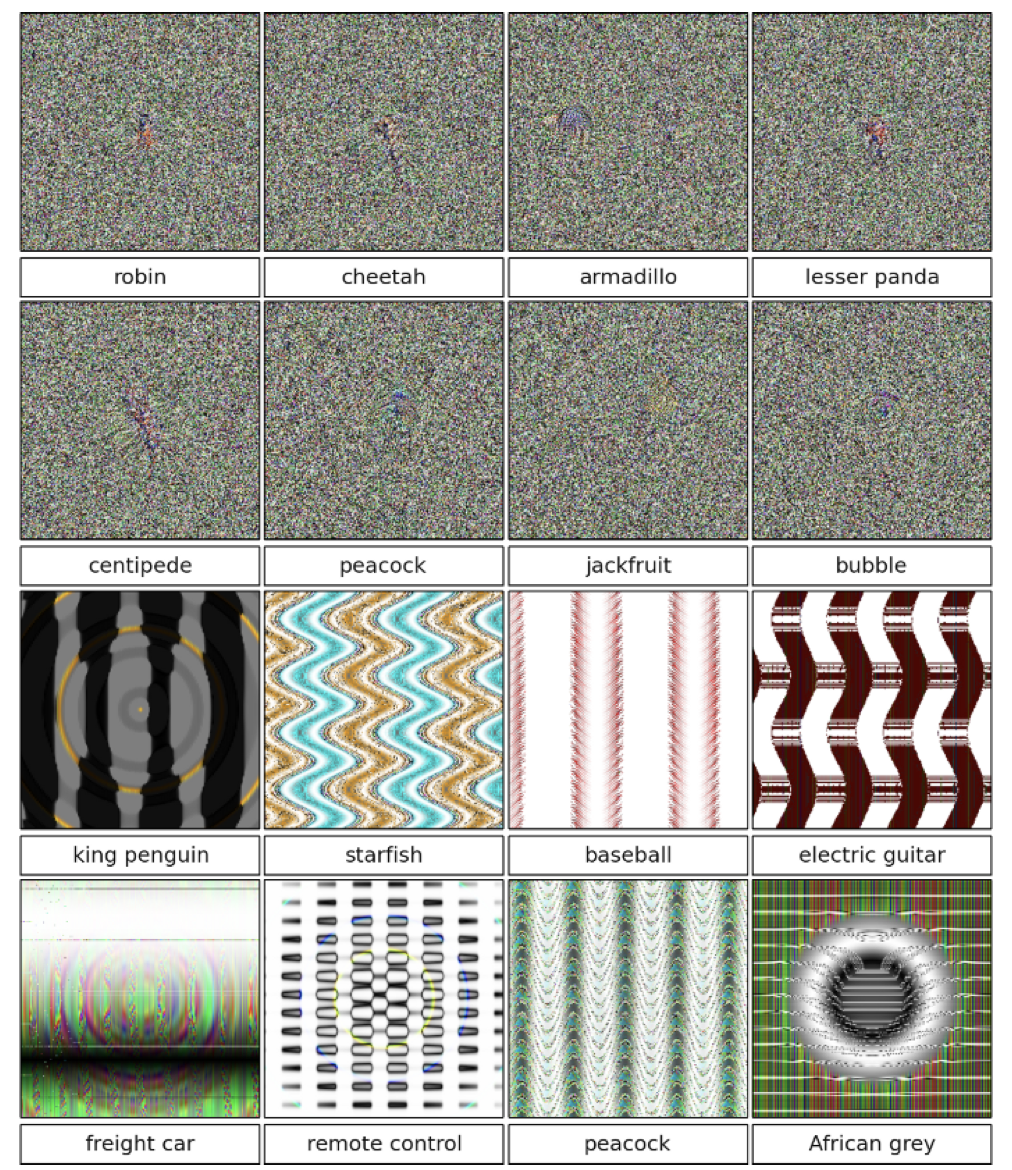
\includegraphics[scale = 0.4]{img/images_fooling_DNN.png}
    \caption[Differences between how DNNs and humans recognize objects]{This result highlights differences between how DNNs and humans recognize objects. Images are either directly (top) or indirectly (bottom) encoded \cite{nguyen2015deep}}
    \label{fig:fooling_DNN}
\end{figure}

With the help of the five factors we studied before, we can further categorize uncertainty in two main categories: aleatoric and epistemic uncertainty. \cite{Separation_uncer}

\begin{figure}[htb]
    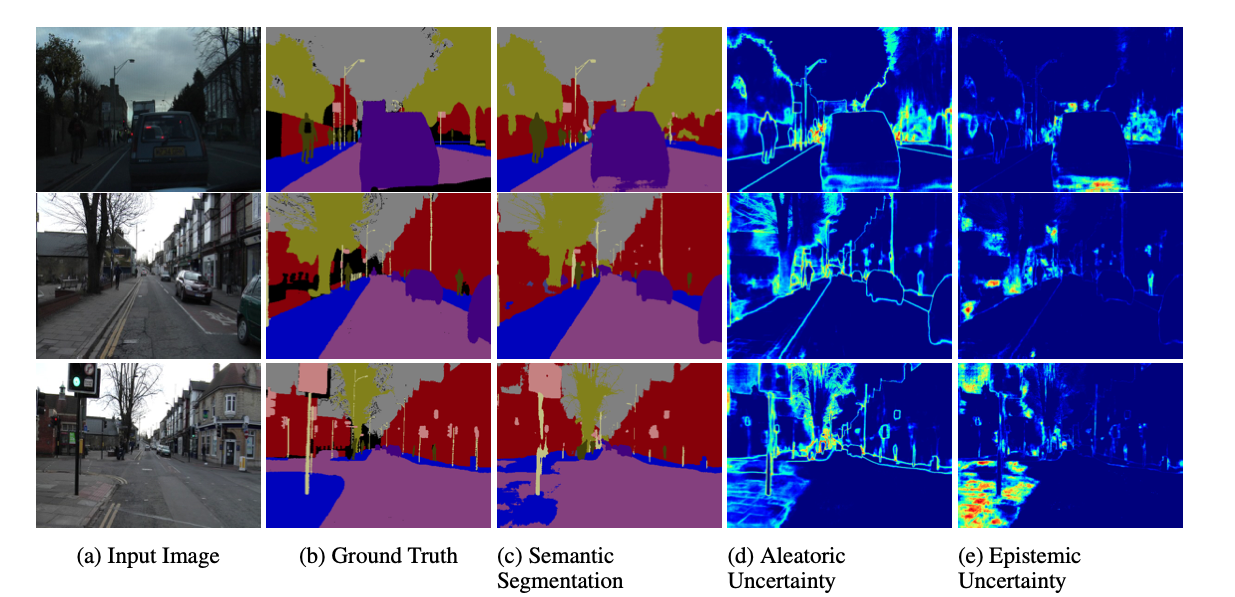
\includegraphics[scale = 0.4]{img/uncert_visua.png}
    \caption[Illustrating the difference between aleatoric and epistemic uncertainty]{Illustrating the difference between aleatoric and epistemic uncertainty for semantic segmentation on the CamVid dataset \cite{DBLP:journals/corr/abs-1811-01412}}
    \label{fig:un_visua}
\end{figure}

\textit{Aleatoric uncertainty} is also usually referred to as data or statistical uncertainty) and it is generally used to identify the type of uncertainty cause by the nature of randomness, that is \textit{ the variability in the outcome of an experiment which is due to inherently random effects} \cite{Separation_uncer}. Moreover, it also comprises the type of noise directly stemming from the noise in data used to train, validate, test and for inference, therefore referring to factor II \cite{gawlikowski2021survey} \cite{DBLP:journals/corr/abs-1811-01412}.  \\
Aleatoric uncertainty is of the irreducible type, meaning it is impossible to get rid of.(\cite{DBLP:journals/corr/KendallG17}, \cite{Separation_uncer}) For example, a model that predicts the output of a flip coin, even in case of a perfect model, is not able to produce the definite, correct answer for it, but only a prediction of the possibilities for the two outcomes. This is due to the fact that the data used for this model is of random, stochastic nature and this random component can not be reduced. \cite{Separation_uncer}\\
\textit{Epistemic uncertainty}, or systemic or epistemic uncertainty, on the other hand, refers to the type of uncertainty cause by ignorance or short comings of the model, hence not on any other underlying stochastic phenomenon. \cite{DBLP:journals/corr/abs-1811-01412}. Usually, this is due to unknown or lack of coverage of the dataset used for training, hence covers factors I,III, IV and V. \\
Epistemic uncertainty can be theoretically explained away by improving the architecture of the model and broadening the dataset.
For example,let us consider a model which is able to determine whether a word is part of the Italian or English dictionary. If we feed the word 'macchina'' to the model, given that we provided enough data to train and the model is perfect, we can be confident that it will predict the correct language, in this case Italian. However, if we feed it with the word ''pasta'', we can not be confident that the prediction is correct, i.e. we can only obtain the probability of this word to be part of one of the dictionaries \textbf{given the dataset we provided}. As a matter of fact, the word ''pasta'' is present in both dictionaries and the outcome depends on the probability of the word to appear in one of the dictionaries in our dataset. The first case is clear case of epistemic uncertainty, which we were able to completely remove with a perfect dataset; while the second case is a clear case of aleatoric uncertainty and it is impossible to remove. 
Fig. \ref{fig:un_visua} helps visualize the difference between the two. In pictures (\textit{d}), we can see that the aleatoric uncertainty increases on object boundaries and objects far from the camera. Pictures (\textit{e}), on the other hand, shows how epistemic uncertainty increases for semantically and visually challenging pixels. For example, the bottom row shows a failure case when the model fails to segment the footpath due to high epistemic uncertainty, but low aleatoric uncertainty. \cite{DBLP:journals/corr/KendallG17}\\
Although this distinction is very helpful for further and more precise analysis on a DNN model, it is also important to note that the distinction between the two is highly dependent on the context: they are not absolute notions.(\cite{KIUREGHIAN2009105}) Hence, changing the settings of the model will blur the distinction line between the two and therefore make their classification considerably more difficult.\cite{Separation_uncer}\\
We mentioned previously that theoretically model uncertainty is 100\% reducible. However, in case of real world data this is not the case. In addition to the probabilistic nature of the DNNs, the training dataset used for the model is very likely to be only a subset of all possible input data of the application, hence it is also very likely that unknown data for the domain is unavoidable. In addition, represent exactly the uncertainty of the DNN is not possible, as the different sources of uncertainty can not be generally modelled accurately. \cite{gawlikowski2021survey}\\

Fur the purpose of this paper, we are not going to explore methodologies to reduce this uncertainty nor we are going to investigate any further whether this uncertainty can be predict from other properties. Our goal will be to research whether we will be able to correlate the other metrics in a way that we can be predictable in time, meaning whether we can define certain time frame for training or inference based on the other characteristics we are going to define. 
%\subsubsection{Modelling Uncertainty}
%\subsection{Classification of uncertainty}

%\subsection{Quantification of uncertainty}

%For a desired degree of confidence (namely, foir a given probability), a confidence interval is a prediction of the range of the output of a model where the actual value exists. With an assumption of a normal distribution of the errors, confidence intervals can be calculated for neural networks.\cite{Confidence_Interval}
%\subsection{Calibration of Neural Networks}
%\subsection{Final remarks on Uncertainty}


\section{Learning Process and Training Time}\label{sec:training_time}
Training time, as the name implies, is the time required to train a Neural Network, or any machine learning model to perform a specific task. \textit{Mitchell} in \cite{machine_learning} provides a general definition for the training, or learning, process : \textit{“A computer program is said to learn from experience E with respect to some class of tasks T and performance measure P, if its performance at tasks in T, as measured by P, improves with experience E.”} This definition is quite broad (\cite{Goodfellow-et-al-2016}) and it is out of the scope of this paper to give a formal definition for the experience E, task T, and performance measure P.\\When it comes to Neural Networks, the process of training is the process of updating the weights of the network so that the network is able to achieve the desired goal. \cite{murphy2016overview} \\
The network weights are updated during back propagation by the following equation(\cite{murphy2016overview}):
\begin{equation}
W = W_{old} - \eta \frac{dE}{dW_{old}}
\label{eq:weigth_updates}
\end{equation}
Equation \ref{eq:weigth_updates} implies that the new value for the weights $W$ is obtained by the difference between the old value $W_{old}$ and the gradient of $W$ of the error function $E$ multiplied by the learning rate $\eta$. The learning rate is a tuning parameter that determines the step size at each iteration while moving towards a minimum of the error function, as we are moving opposite to the gradient. 
The error, or ''scoring'', function can be defined as the sum of squared differences between the network's output(equation n. \ref{eq:MSE}) and the correct output and it is applicable when the output is vector, matrix, or tensor of continuous real values (\cite{murphy2016overview}). 
\begin{equation}
E(W,b) = \frac{1}{N} \sum_{i=1}^{N} \frac{1}{2} \vert \vert h_{W,b} (x^{(i)}) - y^{(i)} \vert \vert ^{2}
\label{eq:MSE}
\end{equation}
Equation \ref{eq:MSE} refers to the Mean Squared Error (MSE), a type of error function usually applied to regression problems and it estimates the average squared difference between the actual values $y^{(i)}$ and the predicted values $h_{W,b} (x^{(i)})$. In other types of problems, different error functions are used. We will describe error functions later in the paper. \\
The learning experience can be broadly categorized into two main categories: supervised and unsupervised learning. Roughly speaking, given a dataset $\mathcal{D}$ , an unsupervised learning algorithm aims to learn useful properties of this dataset. In the context of deep learning, we aim to learn the entire probability distribution $p(\mathcal{D})$ that generated the dataset or some useful properties of it. On the other hand, supervised learning implies the use of a dataset $\mathcal{D}$ and an associated value or label $\mathbb{Y}$ to teach the model to predict $\mathbb{Y}$ from $\mathbb{X} \subset \mathcal{D}$, usually by estimating $p(\mathbb{Y} \vert \mathbb{X})$(\cite{murphy2016overview})\\
Usually the learning process proceeds in waves of mini-batches, which allow to avoid both over-fitting and under utilization of GPU’s compute parallelism.\cite{8573476}\\
Finally, the learning process is a memory demanding task, as backward pass and weight updates, operations unique to training, need to save intermediate results in GPU memory (in some cases tens of gigabytes are required). \cite{rhu2016vdnn}\\
Training time is often an overlooked metrics of Neural Network compared to inference(\ref{sec:inference_time_definition}) or accuracy (\ref{sec:accuracy},\cite{8573476}), however, due to the recent growth in applications of Deep Learning technologies in various fields (\cite{bojarski2016end}, \cite{huval2015empirical}, \cite{10.1145/2959100}, \cite{amodei2015deep}) training time is acquiring importance. \cite{8573476}\\

\section{Inference Time}\label{sec:inference_time_definition}
In Machine Learning, therefore in Deep Learning as well, the term \textbf{inference time} is used to indicate the time required for the trained model to make predictions, regardless of the correctness of those. \\
Inference time has attracted a lot of attention in the research field, since execute already trained Neural Networks efficiently is inarguably a still open problem. (\cite{8573476}, \cite{molchanov2017pruning}, \cite{Duarte_2018}, \cite{7900006})\\
Differently from Training Time (section \ref{sec:training_time}), the memory footprint for inference is in the order of Mega-Bytes(\cite{han2016eie}). As a matter of fact, inference is latency sensitive, but computationally less demanding. \cite{8573476}\\

\section{Accuracy}\label{sec:accuracy}
Accuracy is usually one of the most looked after metrics when analysing Neural Network performances(\cite{hendrycks2019benchmarking},\cite{bianco2018dnnsbench}). Accuracy is usually the factor taken into account when the training process is evaluated, as could be a potential factor deciding when to stop it. Being able to predict accuracy, for example, could help detecting, and therefore terminate, unsuccessful training run \cite{unterthiner2021predicting}. \\
 Usually, the term ''accuracy''  refers to the \textit{classification accuracy} of the neural network. The classification accuracy is the ratio of the number of correct predictions to the total number of input sample (\cite{hussein}) and it is calculated with equation n. \ref{eq:cla_acc}.
\begin{equation}
Accuracy = \dfrac{Number\;of\;correct\;predictions}{Total\;number\;of\;predictions}
\label{eq:cla_acc}    
\end{equation}

In case of a multi-class prediction problem, however, classification accuracy is meaningful only when each class contains an equal number of samples. For example, considering two classes $A$ and $B$ containing 98\% and 2\% of the samples respectively, the model can reach 98\% accuracy by predicting exclusively samples from class $A$. \\
Another definition which is often used for accuracy in Neural Networks in the context of \textit{binary classification} is the one showed in equation n. \ref{eq:bin_acc}.
 \begin{equation}
Accuracy = \dfrac{TP+TN}{TP+TN+FP+FN}
\label{eq:bin_acc}    
\end{equation}
Where TP = True Positives, TN = True Negatives, FP = False Positives, and FN = False Negatives. This equation defines accuracy as the proportion between correctly predicted values (true positives and true negatives) and the sum of all predictions, regardless of their correctness. \\
Similarly to classification accuracy, however, this definition could be misleading as well.  For example, considering a model that classified 100 tumors as malignant (the positive class) or benign (the negative class) as shown in table \ref{tab:tumor}. 

\begin{table}[h]
\centering
\begin{tabular}{ p{1cm} p{2cm} p{2cm} p{2cm}}
 TP&FP&FN&TN\\
 \hline
    1 & 1& 8& 90\\
\end{tabular}
\caption{Example for binary classification}
\label{tab:tumor}
\end{table}
Calculating the accuracy using equation n. \ref{eq:bin_acc}. will give an accuracy of :
 \begin{equation}
Accuracy = \dfrac{1+90}{1+90+1+80} = 0.91
\label{eq:bin_acc2}    
  \end{equation}
At first glance, this metric would show that the model is performing correctly (91 correct out of a 100). The dataset is composed of 91 tumors that are benign (90 TNs and 1 FP) and 9 that are malignant (1 TP and 8 FNs). The model is able to identify 90 out of 91 benign tumors correctly, but only 1 out of 9 as malignant. This is another case of class-imbalanced data set in which a model that would only classify tumors as benign would reach the same level of accuracy. \cite{google_doc}\\



\section{Precision and Recall}
As we already delineated in the previous section, sometimes analysing only at accuracy might be misleading, especially when we are dealing with class-imbalanced data-sets. Accuracy does not distinguish between the number of correct labels of different classes. \cite{metrics} In these cases, two other metrics we can observe are \textit{precision} and \textit{recall}. \\
Formally, \textit{precision} is defined as equation n. \ref{eq:pre} and it represents the number of detected anomalies that are actual real anomalies.\cite{tatbul2019precision}
In other words, it expresses the proportion of positive identifications that was correct over the number of correct predictions. 
\begin{equation}
Precision = \dfrac{TP}{TP+FP}
\label{eq:pre}    
\end{equation}
Where TP = True Positives and FP = False Positives. \\
On the other hand, \textit{recall} is defined as equation n. \ref{eq:rec} and it represents the number of real anomalies that have been detected.\cite{tatbul2019precision}
\begin{equation}
Recall = \dfrac{TP}{TP+FN}
\label{eq:rec}    
\end{equation}
Where TP = True Positives and FN = False Negatives. It is calculated, therefore, as the proportion of positive predictions that were correct over the correct positive predictions and the incorrect negative identifications.  \\
We can use the example in table \ref{tab:tumor} to calculate both precision and recall. 
\begin{equation}
\begin{aligned}
Precision &= \dfrac{TP}{TP+FP}\\
          &= \dfrac{1}{1+1}\\
          &= \dfrac{1}{2}\\
          &= 0.5
\end{aligned}
\label{eq:pre_ex}    
\end{equation}
Having a precision of 0.5, our model is correct 50\% of the time when it predicts that a tumor is malignant. 
\begin{equation}
\begin{aligned}
Recall &= \dfrac{TP}{TP+FN}\\
          &= \dfrac{1}{1+8}\\
          &= \dfrac{1}{9}\\
          &= 0.11
\end{aligned}
\label{eq:rec2}    
\end{equation}
In other words, with a recall of 0.11, our model has been able to identify 11\% of all malignant tumors. \\
Ideally, we would like to have a high recall percentage as well as a high precision one. Unfortunately, this is rarely the case since improving recall often comes at the expense of precision, since in order to increase the TP for the minority class, the number of FP is also often increased, resulting in reduced precision. \cite{10.5555/2559492}\\
Furthermore, as it was the case for accuracy, neither precision nor recall give a full insight on the performance of the model, since a model could have high precision with low recall, as shown in the example above. It is, therefore, common practice to combine both with a weighted harmonic mean as an F score \cite{Rijsbergen1974FOUNDATIONOE}:
\begin{equation}
F_\beta = (1+ \beta ^2)\dfrac{Precision * Recall}{\beta ^2* Precision + Recall}
\label{eq:f_score}    
\end{equation}
In equation n. \ref{eq:f_score}, the coefficient $\beta$ represents the balance between Precision and Recall, with high values favouring Recall. Usually, the F-score is used with $\beta =1$, so a perfect balance between Precision and Recall, and in this case it is called F1 score(Equation n. \ref{eq:f1_score}). \cite{derczynski-2016-complementarity}
\begin{equation}
F1 = (2)\dfrac{Precision * Recall}{Precision + Recall}
\label{eq:f1_score}    
\end{equation}
When evaluating the F score, however,the focus is given exclusively to true positives, false positives and false negatives, neglecting the true negative group, which is usually the majority class. In addition, using the F score, one is unable to distinguish low-recall from low-precision systems. \cite{derczynski-2016-complementarity}\\
\section{Loss}
When training a Neural Network, finding the perfect weights for the neurons is impossible, therefore the problem is usually modelled as an optimization problem. As an optimization problem, it is solved using an algorithm which aims to optimize the weights to make good predictions. Usually, Neural Networks are trained using the Stochastic Gradient Descent (SGD) and the weights are updated through back-propagation. In the context of an optimization algorithm, the function which evaluates a candidate solution is defined as the objective function and such function in Neural Networks evaluates how good a prediction is, hence the SGD is used to minimize this function, i.e. finding the solution with the lowest score. 
When we are minimizing the objective function, we are referring to it as the cost function, loss function, or error function.\cite{Goodfellow-et-al-2016}\\
The loss function has the fundamental job of faithfully distill all the aspects of the model, both good and bad, down into a single, scalar value, which allows candidate solutions to be compared. \cite{reed_neural_1999}\\
The choice of the loss function is highly influenced by the output layer of the Neural Network. The output layer defines the type of the solution we defined for the problem, i.e. if it is a regression problem of a classification problem. In other words, the way we  represent the output determines the loss function. \cite{Goodfellow-et-al-2016}\\
The following are some of the best practices for each type of problem. 

\begin{description}
  \item[Regression problem] \hfill\\ 
  For these type of problems, usually the output layer is one node with a linear activation unit, therefore the loss function to use is the Mean Squared Error(MSE). 
  \item[Binary Classification problem] \hfill\\ 
  The output layer is one node with a sigmoid activation unit and the loss function used is Cross-Entropy, or Logarithmic loss. 
  \item[Multi-class Classification problem] \hfill\\ 
  The output layer is composed of one node for each class using the soft-max activation function nd the loss function used is Cross-Entropy, or Logarithmic loss. 
\end{description}


%\cite{10.5555/525960}



%\url{https://machinelearningmastery.com/loss-and-loss-functions-for-training-deep-learning-neural-networks/}

\section{Overfitting and Underfitting }\label{sec:of_uf}
As we already discovered in section n. \ref{sec:training_time}, the training routine is necessary for the model in order to make predictions on a new set of data. Therefore, the goal of the learning process is not to minimize the accuracy on the training set, but rather to maximize its predictive accuracy on the new data points. \citep{dietterich1995overfitting}\\
If the model works too hard to find the best fit for the training data there is the risk that it is going to fit the noise present on the data-set, hence it will learn the inevitable peculiarities and bias present in the training set, rather than finding a general predictive rule. In other words, the performance of the model will decrease when tested against an unknown data-set.\cite{jabbar2015methods} This phenomena is called \textit{over-fitting}. \citep{dietterich1995overfitting}\\
Over-fitting is influenced by the training data fed to the model, as small data-sets are more prone to it, even though also large data-sets can be affected. \cite{10.1016/j.inffus.2008.11.003}\\
Under-fitting, on the other hand, can be considered as the opposite process. This occurs when the model is too simple for the training data and it is incapable of learning the variability of the data. \cite{10.1016/j.inffus.2008.11.003}\\

One strategy to avoid over-fitting is to use a so-called ''early-stopping'' approach. This approach consists simply of stopping the training before over-fitting can occur and it is one of the mostly used strategies to avoid this phenomena, as it is simple to understand and proven to be the superior one in many cases (\citep{FINNOFF1993771}, \cite{early_stopping}). \\
The key part of this approach is to divide the training set into two parts, namely the validation set and the training set, and to use those to find a criteria to stop the training process. \\
Fig. \ref{fig:over_fitting_curve} shows the idealized evolution over time of the error on the training set and on a validation set not used for training, i.e. training and validation loss.\cite{early_stopping}

\begin{figure}[htb]
    \centering
    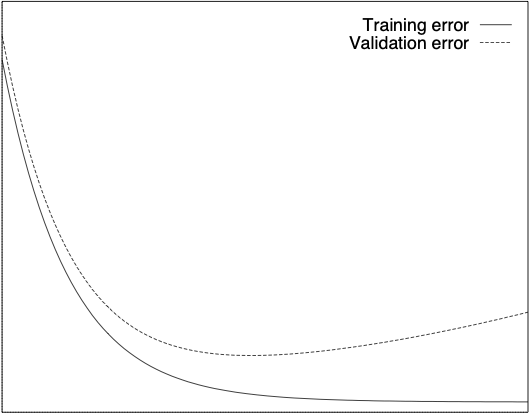
\includegraphics[scale = 0.3]{img/over_fitting.png}
    \caption[Validation and training loss curve]{Validation and training loss curve. The x axis is time, the y axis is the loss \cite{early_stopping}}
    \label{fig:over_fitting_curve}
\end{figure}


Following the trend in Fig. \ref{fig:over_fitting_curve}, we can observe that the validation error decreases until a certain point together with the training loss before increasing indefinitely. We can use the validation error to approximate the generalization error and, therefore, stop the training in the moment where the validation loss is increasing again. 
We can summarize the ''early-stopping'' approach in the following steps:
\begin{enumerate}
\item Split the training data into a training set and a validation set, for i.g. in a 4-to-1 proportion
\item Train over the training and evaluate the validation loss every arbitrary number of epoch
\item Stop training as so on as the error on the validation set is         higher than it was last time
\item Use the weights the network had in that previous step as the result of the training run

\end{enumerate}
Furthermore, depending on the data, there might be also situations in which the validation loss is not constantly bigger than the training loss, as shown in Fig. \ref{fig:over_fitting_curve}. As a matter of fact, this graph shows an idealized behaviour of the two curves. A real example for this curve can be seen in Fig. \ref{fig:over_fitting_curve_real}.
\begin{figure}[htb]
    \centering
    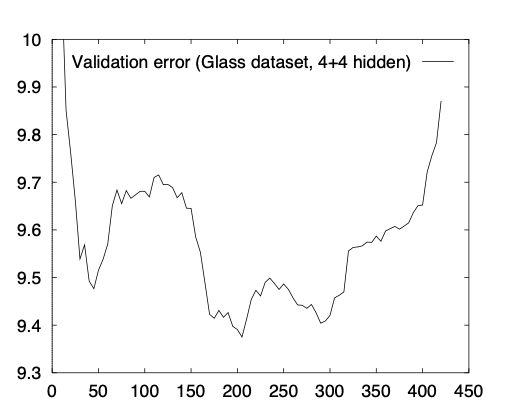
\includegraphics[scale = 0.4]{img/over_fitting_real.png}
    \caption[Real Example of the Validation and training loss curve]{Real Example of the Validation and training loss curve. The x axis is time, the y axis is the loss \cite{early_stopping}}
    \label{fig:over_fitting_curve_real}
\end{figure}

In such situations, it would be particularly difficult to choose an optimal stopping criteria, as the validation function as multiple local minima (16 in the pictures case). It is left to the reader to investigate strategies to optimize early-stopping in these situations. \\
Furthermore, there are also scenarios in which, depending on the data presented, the validation loss is at first less than the training loss, as shown in Fig. \ref{fig:over_fitting_curve_2}. 
\begin{figure}[htb]
    \centering
    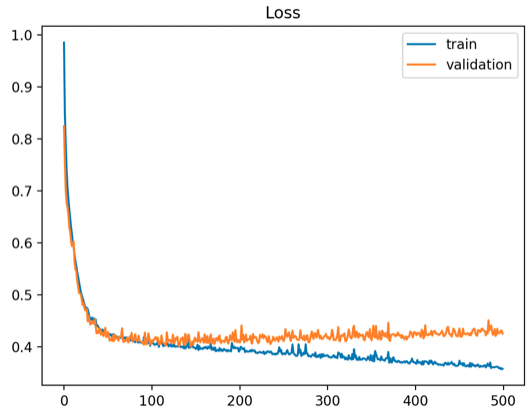
\includegraphics[scale = 0.4]{img/over_fitting_2.png}
    \caption[Real Example of the Validation and training loss curve]{Real Example of Validation and training loss curve. The x axis is time, the y axis is the loss}
    \label{fig:over_fitting_curve_2}
\end{figure}

In these situation, as a rule of thumb, we can use the following statements to determine the status of the training and decide when to stop. 
\begin{itemize}
\item validation loss $>>$ training loss: over-fitting
\item validation loss $>$ training loss: some over-fitting
\item validation loss $<$ training loss: some under-fitting
\item validation loss $<<$ training loss: under-fitting

\end{itemize}


\section{Architecture}\label{sec:arch}
In the following sections we are going to briefly analyse the architectures of the models we are going to study to find characteristics and correlations. \\
For the sake of this paper, we are going to limit our analysis to some of the most common architectures for convolutional neural networks which have been proven by other studies (\cite{suh_transfer_2018}, \cite{s20205893}, \cite{phdthesis}) to achieve promising results in the settings of sugar beet recognition. The architecture chosen are listed below and are treated in more details in their respective sections. 
\begin{itemize}
\item Resnet
\item Alexnet
\item VGG
\end{itemize}
\subsection{Alexnet}
Alexnet is a Convolutional Neural Network (CNN) architecture designed by  Alex Krizhevsky in collaboration with Ilya Sutskever and Geoffrey Hinton. \cite{NIPS2012_c399862d}\\
The architecture is depicted in Fig. \ref{fig:alexnet_architecture}. The net is composed of eight layers:
The first 5 are convolutional layer an convolutional and the remaining three are fully- connected. The output of the last fully-connected layer is fed to a 1000-way Softmax which produces a distribution over the 1000 class labels. \cite{NIPS2012_c399862d}\\
\begin{figure}[htb]
    \centering
    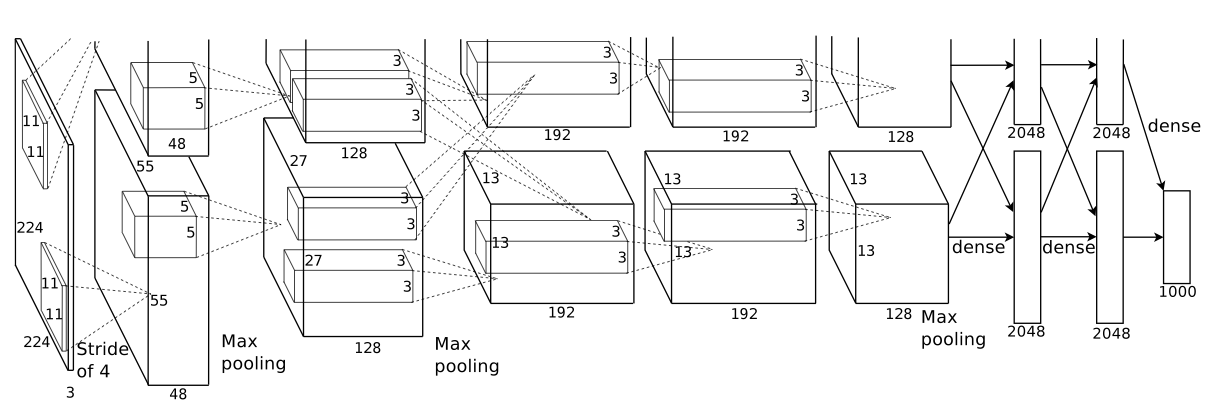
\includegraphics[scale = 0.4]{img/alexnet_architecture.png}
    \caption[Overview of the architecture of Alexnet]{Overview of the architecture of Alexnet \cite{NIPS2012_c399862d}}
    \label{fig:alexnet_architecture}
\end{figure}


As described by \textit{Krizhevsky et al.} in \cite{NIPS2012_c399862d}, the layers are defined as it follows:

\begin{itemize}
\item The first convolutional layer receive as input a 224 × 224 × 3  image and filters it with 96 kernels of size 11 × 11 × 3 with a stride of 4 pixels\footnote{The stride is the distance between the receptive field centers of neighboring neurons in a kernel map}
\item The second convolutional layer takes as input the response-normalized and pooled output of the first layer and filters it with 256 kernels of size 5 × 5 × 48.
\item The third layer has 384 kernels of size 3 × 3 × 256 it is connected to the normalized and pooled output of the second
\item The fourth convolutional layer has 384 kernels of size 3 × 3 × 192 and it is connected to the third without pooling or normalization layers
\item The fifth convolutional layer has 256 kernels of size 3 × 3 × 192 and as input it receives the output of the forth. 
\item The fully-connected layers are composed of 4096 neurons each
\end{itemize}
\subsection{VGG Networks}\label{sec:VGG}
VGG stands for Visual Geometry Group at Oxford University and have been developed by Simonyan and Zisserman in \cite{simonyan2015deep} for the 
ILSVRC (Image Net Large Scale Visual Recognition Challenge) 2014 competition
(\cite{DBLP:journals/corr/RussakovskyDSKSMHKKBBF14}). 
The concept of VGG net is similar to Alexnet: as net increases, the number of convolutions and future maps increases as well. Rather than using 11 × 11 feature detectors or filters, however, the authors decided to use smaller 3 x 3  filters. The various architecture proposed in \cite{simonyan2015deep} are showed in Fig. \ref{fig:vgg_arch}. In this paper, we are going to consider only the networks D and E, i.e. with 16 and 19 weight layers respectively. For the rest of the paper, we are going to refer to them as VGG16 and VGG19 respectively. 

\begin{figure}[htb]
    \centering
    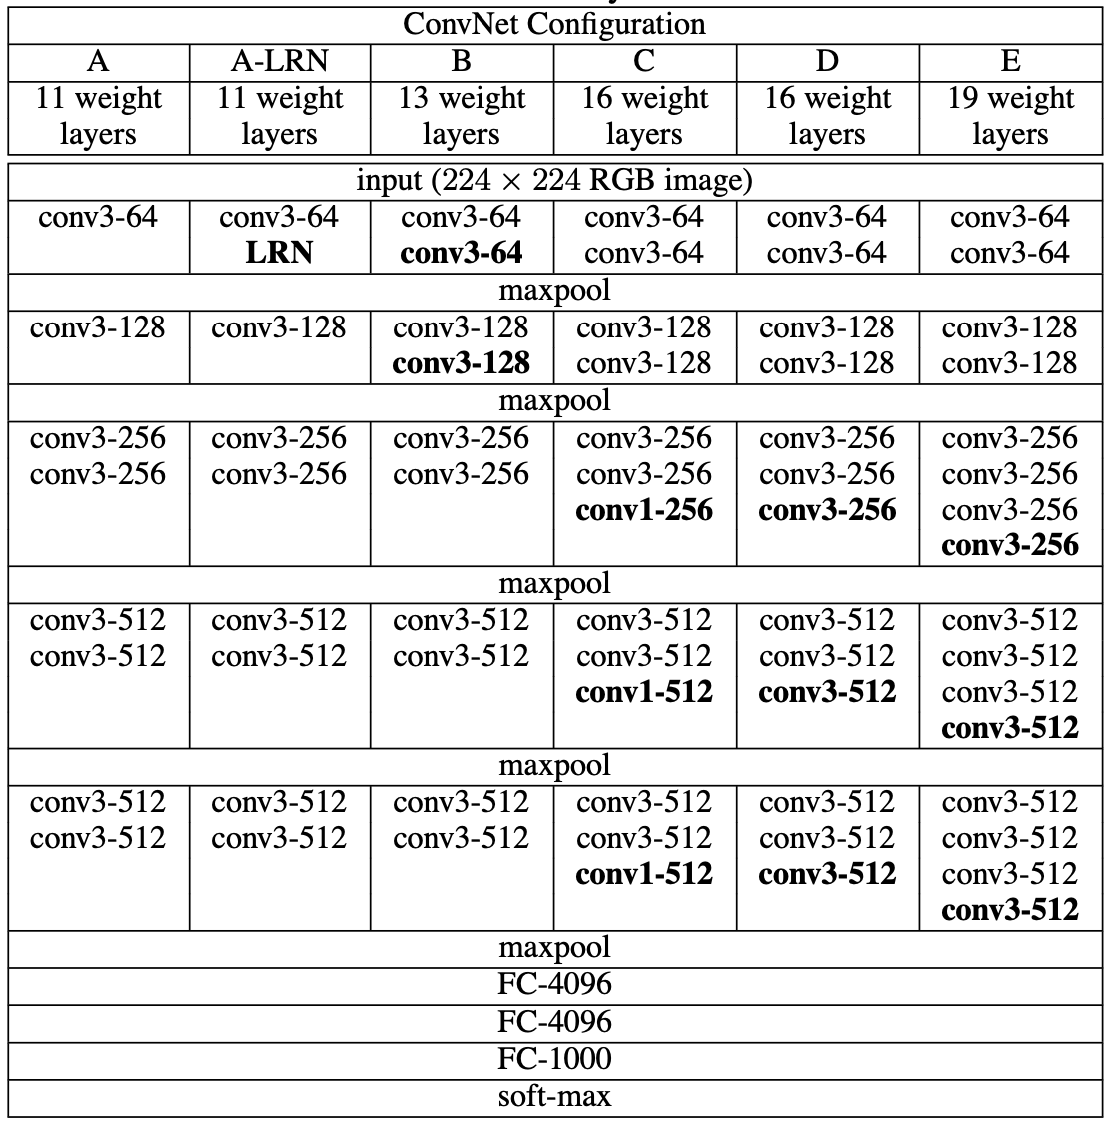
\includegraphics[scale = 0.5]{img/vgg_arch.png}
    \caption[Overview of the various architecture for VGG]{Overview of the various architecture for VGG \cite{simonyan2015deep}}
    \label{fig:vgg_arch}
\end{figure}



%\begin{figure}[htb]
 %   \centering
  %  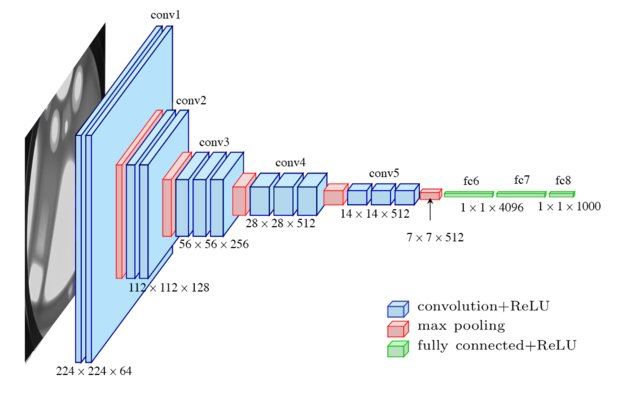
\includegraphics[scale = 0.5]{img/vgg_picture.jpg}
   % \caption[Residual learning: a building block]{\cite{vgg_picture}}
  %  \label{fig:res_block}
%\end{figure}





\subsection[Residual Neural Networks]{Residual Neural Networks (Resnet)}
Many studies (\citep{simonyan2015deep}, \cite{szegedy2014going}) reveal that the depth of the Neural Networks is crucial and for most visual recognition tasks the trend has been to stack more layers into neural networks and increase their depth. (\cite{simonyan2015deep},\cite{ioffe2015batch},\cite{girshick2014rich},\cite{2014Spatial})\\
Training deeper networks like VGG19 and VGG16 (section n.\ref{sec:VGG} ), however, is not a trivial task, since,as they start converging, the accuracy starts to saturate and then degrades quickly. This phenomena is due to the gradient vanishing during back-propagation, i.e. when the weights are updated, as it becomes smaller the more layers it goes through and vanishes before reaching the initial layer, hence they can not be updated.  \\
\textit{He et al. } in \cite{DBLP:journals/corr/HeZRS15} tackle the problem of degradation with the introduction of a \textit{deep residual learning} framework. At the core of the framework there is the so called ''residual block'', shown in Fig. \ref{fig:res_block}. 
\begin{figure}[htb]
    \centering
    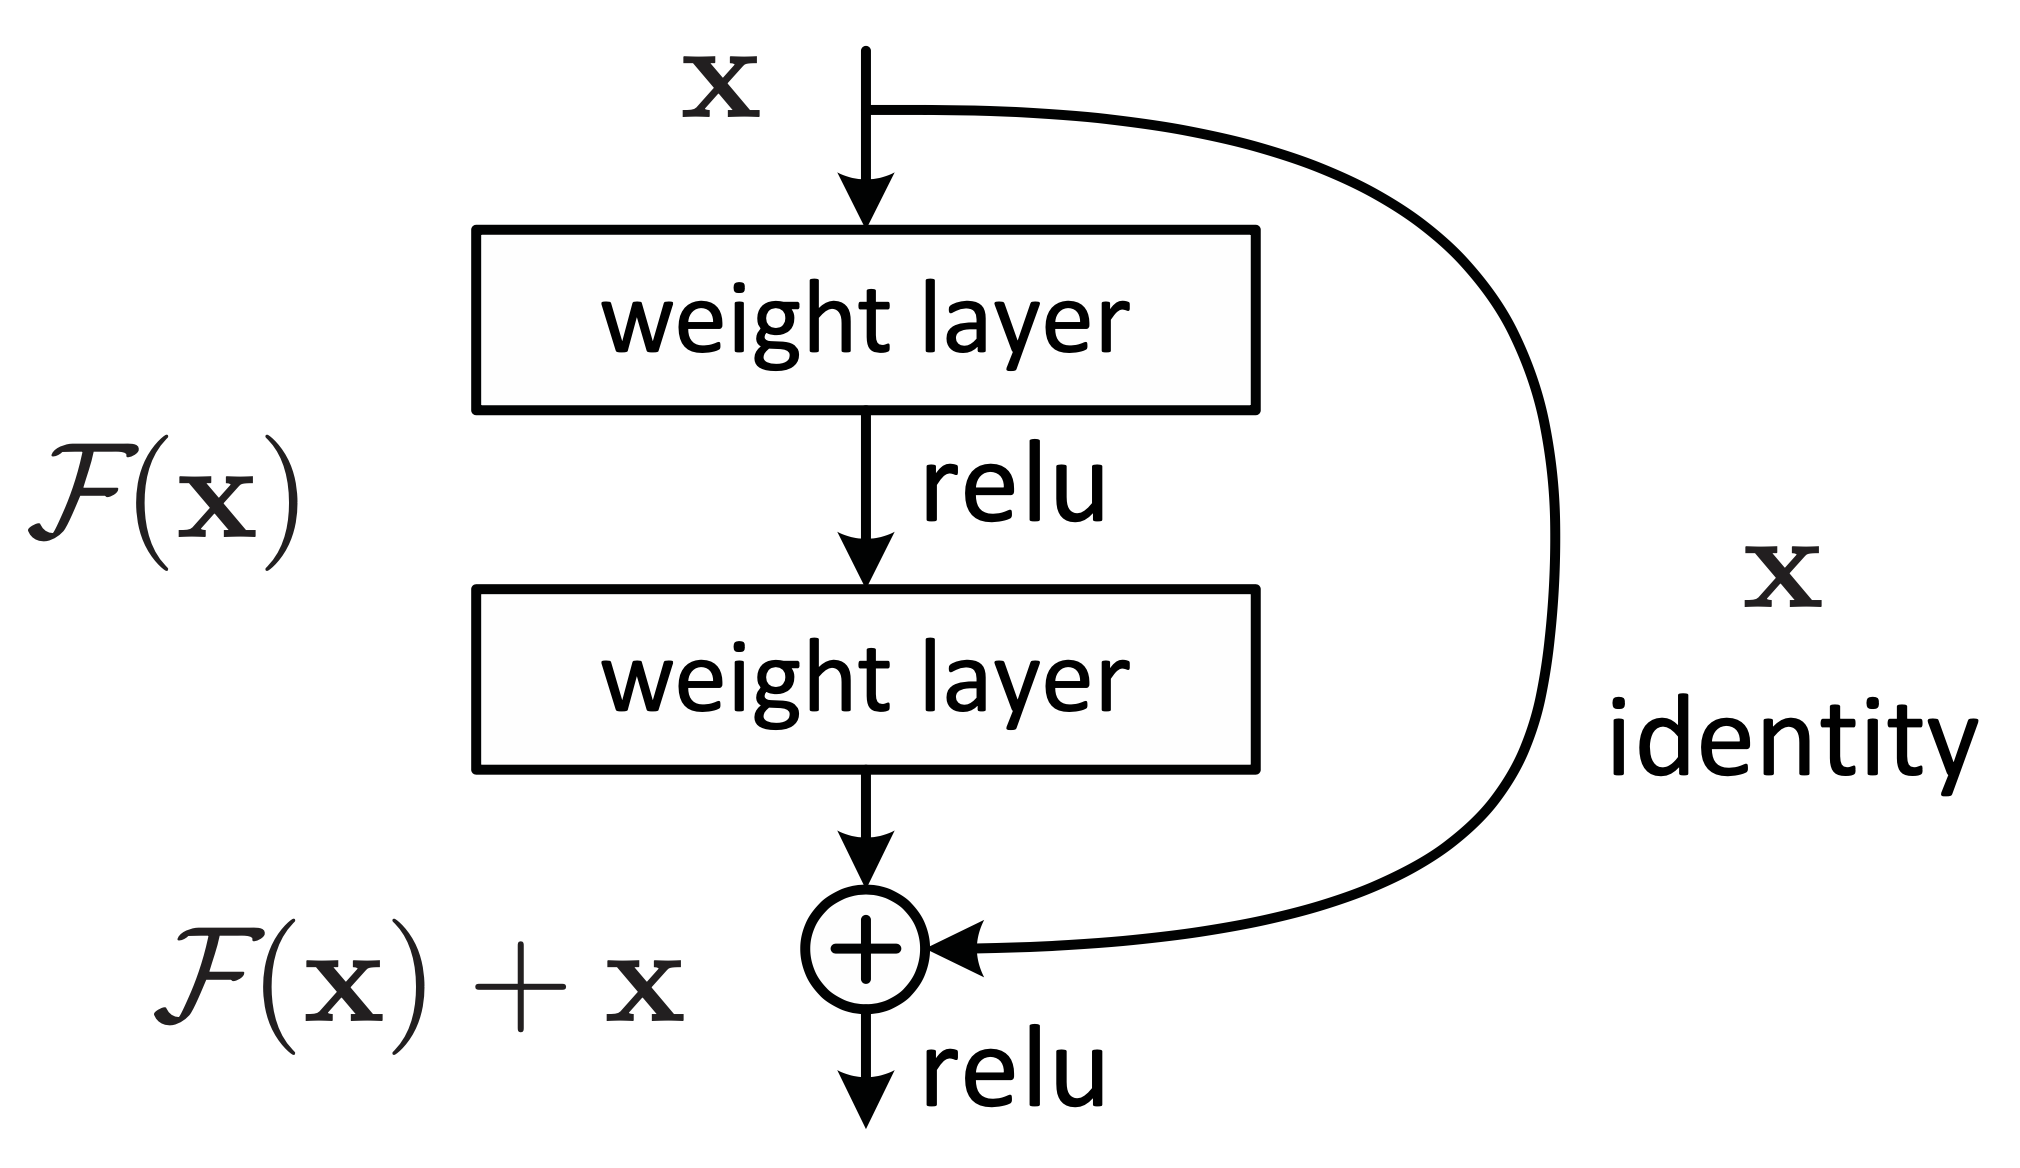
\includegraphics[scale = 0.3]{img/res_block.png}
    \caption[Residual learning: a building block]{Residual learning: a building block. \cite{DBLP:journals/corr/HeZRS15}}
    \label{fig:res_block}
\end{figure}

Differently from plain convolutional networks, these blocks also have the so called ''identity connection'' between the input and the output layer. 
In plain convolutional networks, the output $\mathcal{H}(x)$ is obtained by:
\begin{align*}
\mathcal{H}(x) &= \mathcal{F}(wx + b)\\
               &or\\
\mathcal{H}(x) &= \mathcal{F}(x)\\   
\end{align*}
with $w$ being the weights and $b$ being the bias\\
With the introduction of residual blocks, the output function assumes the form showed in equation n. \ref{eq:residual_blocks}, with $x$ being the input.
\begin{equation}
\mathcal{H}(x) = \mathcal{F}(x) + x
\label{eq:residual_blocks}   
\end{equation}
Reworking the equation lets us obtain the so called \textit{residual function}: 
\begin{equation}
\mathcal{F}(x) = \mathcal{H}(x) - x
\label{eq:residual_function}   
\end{equation}

The purpose of residual networks becomes to approximate the residual function, hence the difference between the input and the output.In other words, the aim is to learn the residual function in a way such that it approaches zero, hence making the identity value optimal. \\
The problem of the vanishing gradient is resolved by the identity function. During back-propagation the gradient can take this path and, since no weights are encountered, there won't be any change in the value computed by the gradient. This effectively allows the gradient to entirely skip the block and reach the initial layers and correct their weights. \\
The architecture of residual networks we are going to use in this paper is showed in Fig. \ref{fig:resnet_arch}. For the rest of the paper, we are going to refer them as ''Resnet'' followed by the amount of layers. For example, Resnet18 refers to the residual network having the 18 layers described in Fig.  \ref{fig:resnet_arch}. 
\begin{figure}[t]
    \centering
    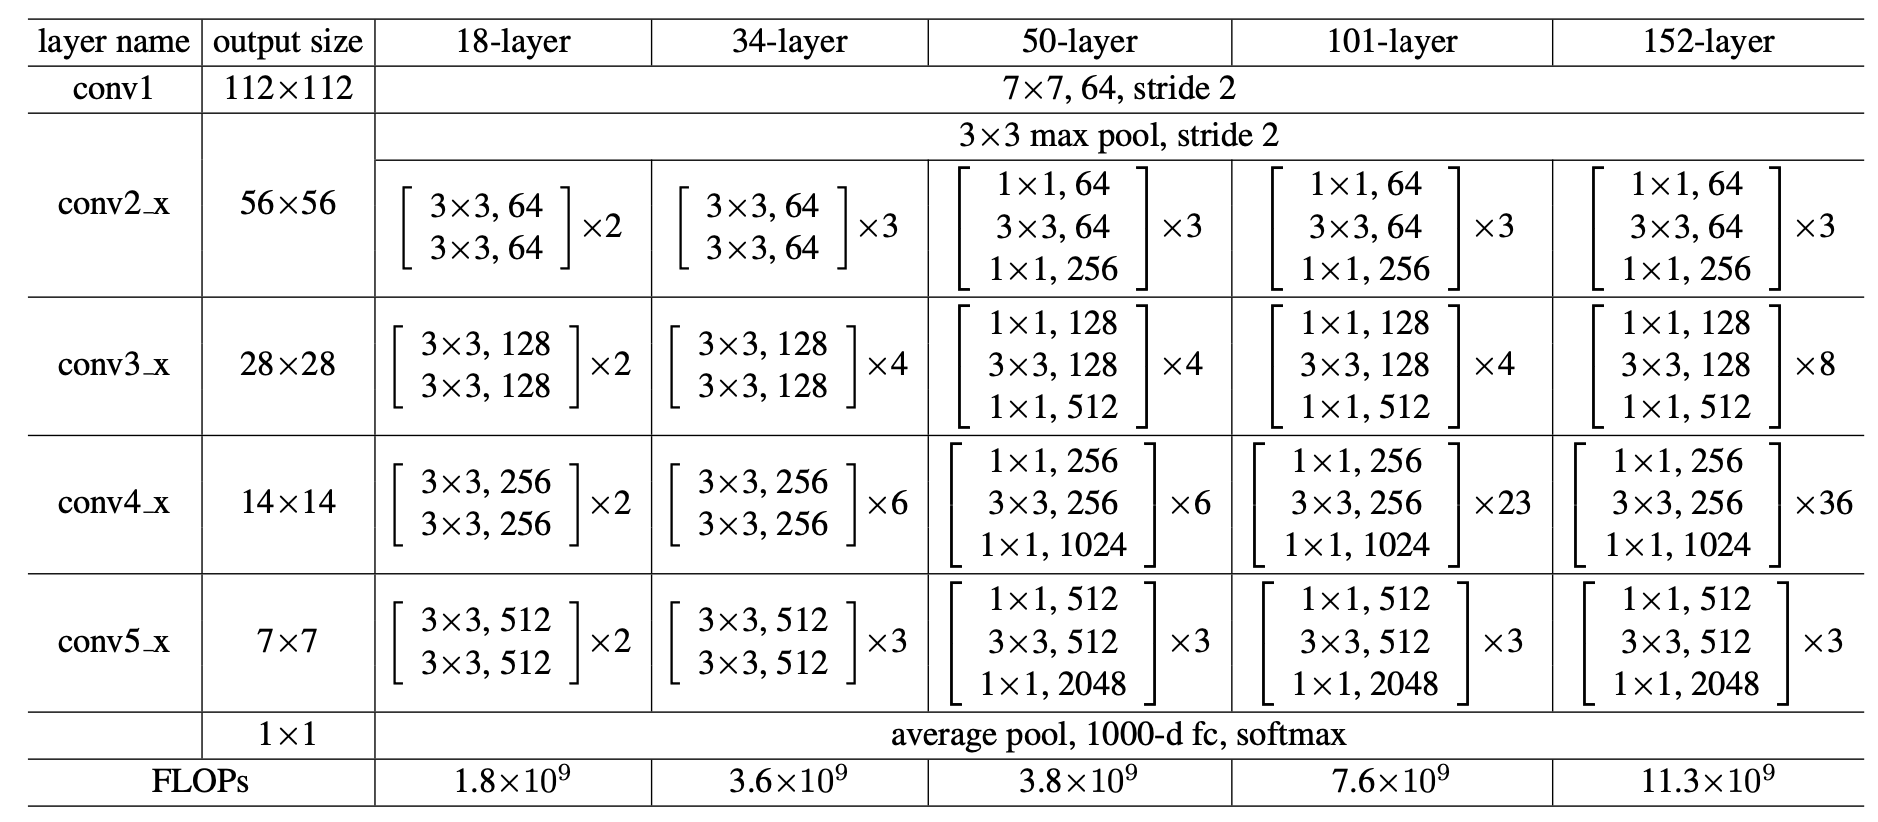
\includegraphics[scale = 0.5]{img/resnet_arch.png}
    \caption[Overview of the Resnet Architecture]{Overview of the Resnet Architecture. The building blocks are shown in brackets \cite{DBLP:journals/corr/HeZRS15}}
    \label{fig:resnet_arch}
\end{figure}


